%!TEX root = ../Hardtung_BA_SoSe20.tex

\section{Problemfield \& Context}

Origami is the Japanese art of folding paper into models of animals, people or other objects. Folding instructions for such origami models are called diagrams (Fig \ref{fig:cranediagram} shows an example of how such a diagram looks like). But as creating these diagrams is a tedious and time consuming process, the Origrammer \cite{origrammer} was developed. The Origrammer is a desktop application, developed by the author, which offers specific features for creating such Origami Diagrams (see Fig. \ref{fig:origrammerMain} for an overview of this program).
This Bachelor Thesis aims to evaluate the current state of this program and to develop it further to improve usability, efficiency and effectivity.

\begin{figure}[h]
\centering
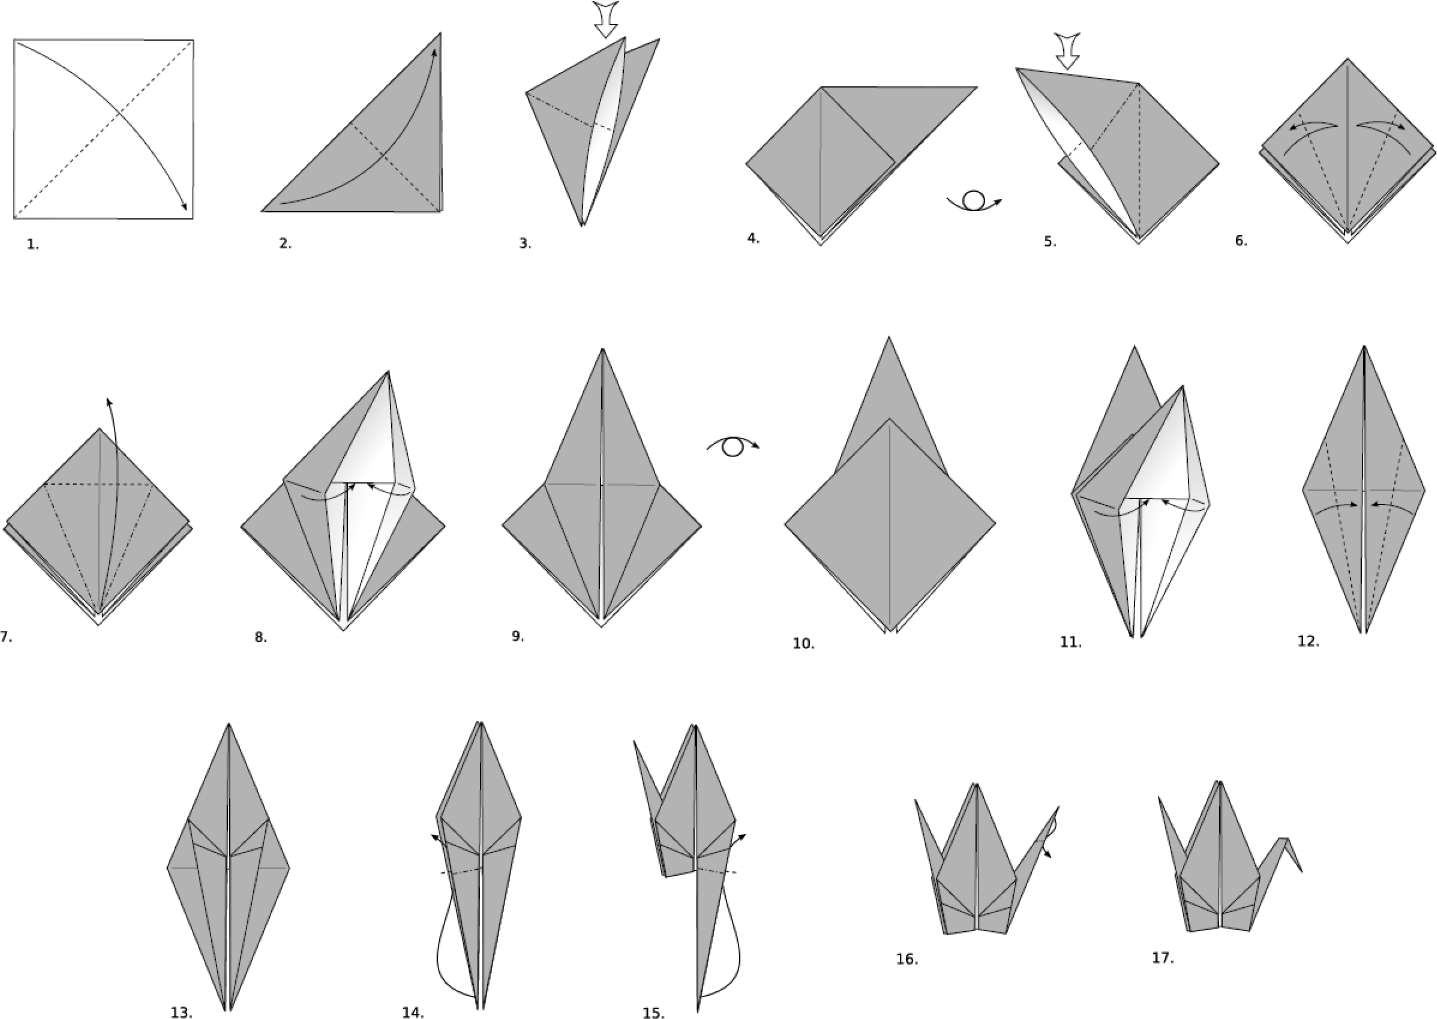
\includegraphics[width=0.75\textwidth]{crane1}
\caption{Origami Diagram Example of a Crane}
\label{fig:cranediagram}
\end{figure}


\begin{figure}[h]
\centering
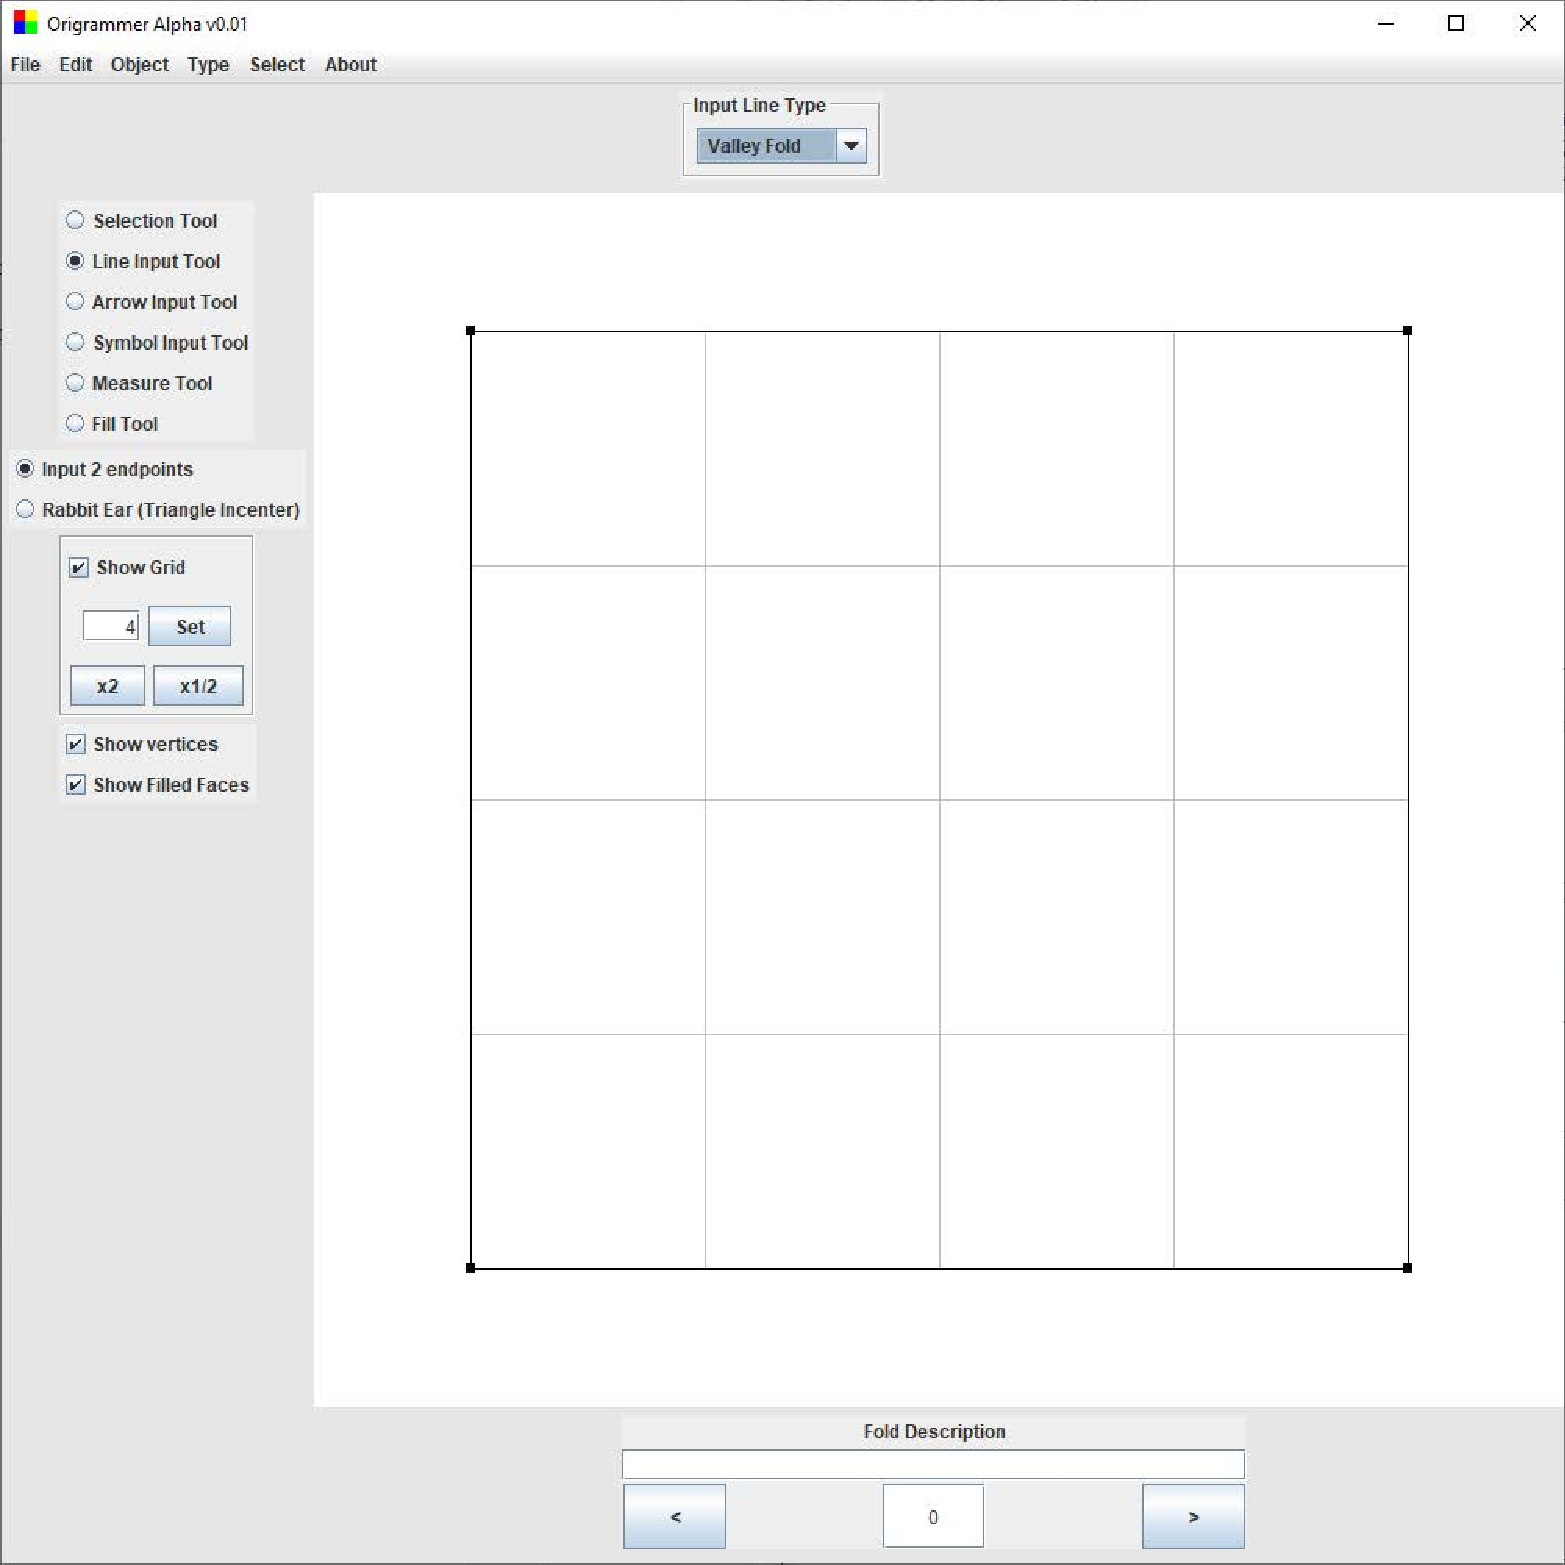
\includegraphics[width=0.6\textwidth]{OrigrammerMain}
\caption{Origrammer}
\label{fig:origrammerMain}
\end{figure}

\newpage

\section{Goal}
The goal of this bachelor thesis is to improve general usability of the Origrammer. In order to achieve this the current state of this program has to be evaluated. Problems and shortcomings will be listed and sorted after severity and potential impact on usability when improving said problems.

The main focus will be set on refining the user interface to make the workflow more straight forward as well as simplifying user inputs. This simplification process should also include a certain grade of automation. This is especially important with the original goal of the Origrammer in mind.
\begin{center}
\enquote{\emph{The goal for this project is to develop a desktop application that implements features specifically for the origami diagramming process. The standardized symbols and overall notations have to be included and the program \textbf{has to offer functions that increase the efficiency of creating diagrams}.}} \cite{origrammer}
\end{center}
Then after evaluating and collecting potential improvements a more detailed plan can be created on how to actually implement these changes. Different possible solutions should be tested for pros and cons and the best solutions should then be developed for the Origrammer.


\section{Ressources}\label{ressourcen}

As this work will focus on the evaluation and improvement of an existing system, most of the relevant ressources will consist of different evaluation methods, as well as current Human-Computer Interaction criteria. 


\section{Chances \& Risks}

The evaluation of an existing system can always entail certain risks. Especially the current (at the time of writing this thesis) Covid-19 pandemic hinders user involvement during this process. Testing with a few selected users could be done with the help of digital methods, but this approach would increase the required time immensely.

However, other measures can be taken to counteract the missing user input. Carrying out inspections with heuristic procedures like the \emph{10 usability heuristics} \cite{usability_heuristics}, which are part of the \emph{discount usability engineering} \cite{discount_usability_engineering} by Nielsen and Molich, can offer an additional perspective without any required real users.


Furthermore the real users could be substituted for personas in some evaluation methods and despite having an existing system, some formative evaluation methods can also be used to discover usability issues.
And by repeating the evaluation process iteratively after the implementation of design solutions, the chance of missing severe usability problems will be reduced even further.

\newpage

\section{Time Schedule}
\begin{figure}[h]
\centering
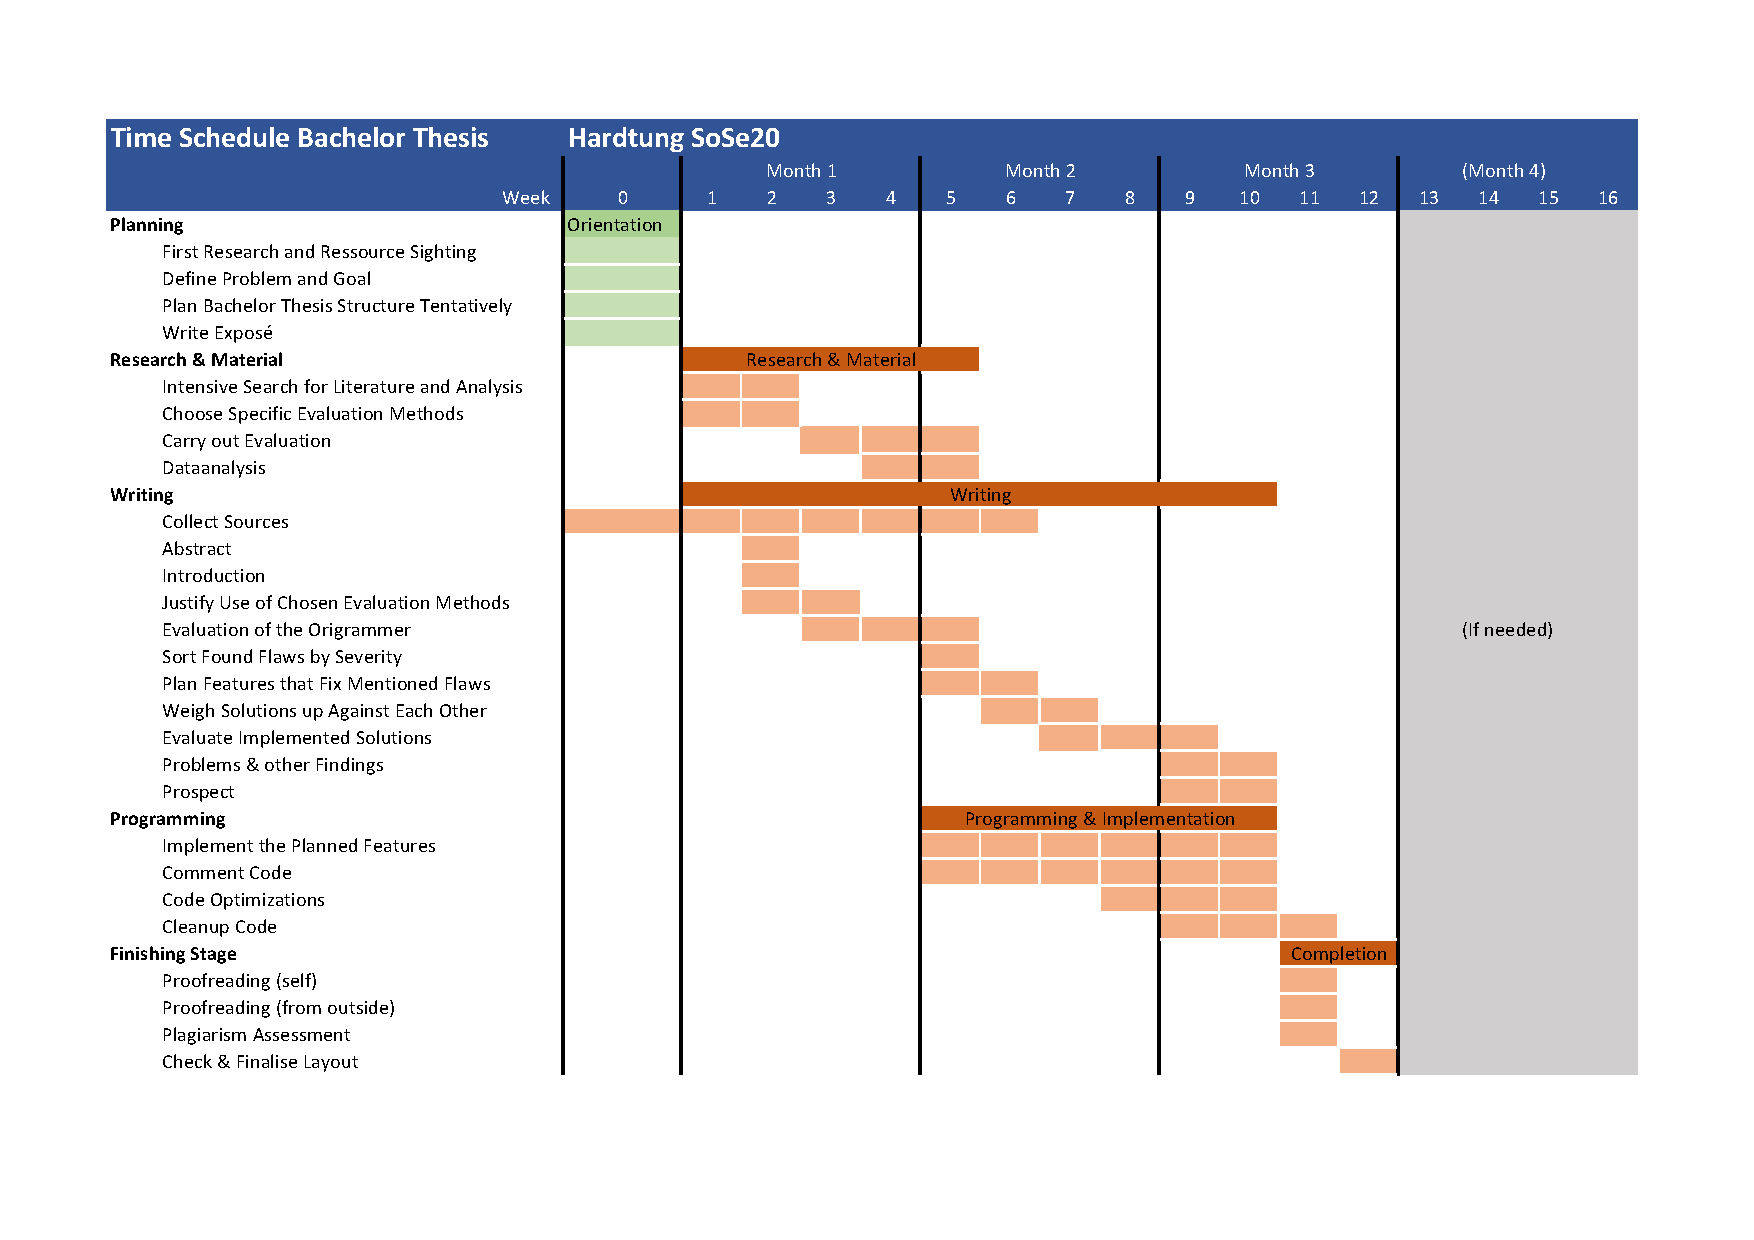
\includegraphics[angle=90,origin=c,width=0.80\textwidth]{TimeSchedule}
%\caption{Time Schedule}
\label{fig:timeSchedule}
\end{figure}
